%%
%% This is file `sample-sigplan.tex',
%% generated with the docstrip utility.
%%
%% The original source files were:
%%
%% samples.dtx  (with options: `all,proceedings,bibtex,sigplan')
%% 
%% IMPORTANT NOTICE:
%% 
%% For the copyright see the source file.
%% 
%% Any modified versions of this file must be renamed
%% with new filenames distinct from sample-sigplan.tex.
%% 
%% For distribution of the original source see the terms
%% for copying and modification in the file samples.dtx.
%% 
%% This generated file may be distributed as long as the
%% original source files, as listed above, are part of the
%% same distribution. (The sources need not necessarily be
%% in the same archive or directory.)
%%
%%
%% Commands for TeXCount
%TC:macro \cite [option:text,text]
%TC:macro \citep [option:text,text]
%TC:macro \citet [option:text,text]
%TC:envir table 0 1
%TC:envir table* 0 1
%TC:envir tabular [ignore] word
%TC:envir displaymath 0 word
%TC:envir math 0 word
%TC:envir comment 0 0
%%
%%
%% The first command in your LaTeX source must be the \documentclass
%% command.
%%
%% For submission and review of your manuscript please change the
%% command to \documentclass[manuscript, screen, review]{acmart}.
%%
%% When submitting camera ready or to TAPS, please change the command
%% to \documentclass[sigconf]{acmart} or whichever template is required
%% for your publication.
%%
%%
\documentclass[sigplan,screen]{acmart}

%%
%% \BibTeX command to typeset BibTeX logo in the docs
\AtBeginDocument{%
  \providecommand\BibTeX{{%
    Bib\TeX}}}

%% Rights management information.  This information is sent to you
%% when you complete the rights form.  These commands have SAMPLE
%% values in them; it is your responsibility as an author to replace
%% the commands and values with those provided to you when you
%% complete the rights form.
\setcopyright{acmlicensed}
\copyrightyear{2024}
\acmYear{2018}
\acmDOI{XXXXXXX.XXXXXXX}

%% These commands are for a PROCEEDINGS abstract or paper.
\acmConference[Cloud computing e infraestructura para Big Data]{Make sure to enter the correct
  conference title from your rights confirmation emai}{Agosto 31-08,
  2024}{Santa Cruz, Bolivia}
%%
%%  Uncomment \acmBooktitle if the title of the proceedings is different
%%  from ``Proceedings of ...''!
%%
%%\acmBooktitle{Woodstock '18: ACM Symposium on Neural Gaze Detection,
%%  June 03--05, 2018, Woodstock, NY}
\acmISBN{978-1-4503-XXXX-X/18/06}


%%
%% Submission ID.
%% Use this when submitting an article to a sponsored event. You'll
%% receive a unique submission ID from the organizers
%% of the event, and this ID should be used as the parameter to this command.
%%\acmSubmissionID{123-A56-BU3}

%%
%% For managing citations, it is recommended to use bibliography
%% files in BibTeX format.
%%
%% You can then either use BibTeX with the ACM-Reference-Format style,
%% or BibLaTeX with the acmnumeric or acmauthoryear sytles, that include
%% support for advanced citation of software artefact from the
%% biblatex-software package, also separately available on CTAN.
%%
%% Look at the sample-*-biblatex.tex files for templates showcasing
%% the biblatex styles.
%%

%%
%% The majority of ACM publications use numbered citations and
%% references.  The command \citestyle{authoryear} switches to the
%% "author year" style.
%%
%% If you are preparing content for an event
%% sponsored by ACM SIGGRAPH, you must use the "author year" style of
%% citations and references.
%% Uncommenting
%% the next command will enable that style.
%%\citestyle{acmauthoryear}
\usepackage{tabularx}
\usepackage{graphicx}
\usepackage[spanish]{babel}

\newcommand{\staricon}[1]{
    \begin{tikzpicture}[scale=#1]
        \filldraw[fill=yellow, draw=black] 
        (0,0) -- (0.2,0.6) -- (0.6,0.6) -- (0.3,0.9) -- (0.4,1.4) -- (0,1.1) -- (-0.4,1.4) -- (-0.3,0.9) -- (-0.6,0.6) -- (-0.2,0.6) -- cycle;
    \end{tikzpicture}
}

%%
%% end of the preamble, start of the body of the document source.
\begin{document}

%%
%% The "title" command has an optional parameter,
%% allowing the author to define a "short title" to be used in page headers.
\title{Visualizers: Athena vs. Looker Studio}

%%
%% The "author" command and its associated commands are used to define
%% the authors and their affiliations.
%% Of note is the shared affiliation of the first two authors, and the
%% "authornote" and "authornotemark" commands
%% used to denote shared contribution to the research.
\author{Bravo Peña}
\author{Darlyn}
\affiliation{
  \institution{UAGRM}
  \city{Santa Cruz}
  \country{Bolivia}
}
\email{contact@bpdarlyn.com}

\author{Torrejón Mendez}
\author{Joel Gabriel}
\affiliation{
  \institution{UAGRM}
  \city{Santa Cruz}
  \country{Bolivia}
}
\email{joel.torrejon.mendez@gmail.com}

\author{Valle Tamayo}
\author{Brandon Jason}
\affiliation{
  \institution{UAGRM}
  \city{Santa Cruz}
  \country{Bolivia}}
\email{bjvtamayo78@gmail.com}
%%
%% By default, the full list of authors will be used in the page
%% headers. Often, this list is too long, and will overlap
%% other information printed in the page headers. This command allows
%% the author to define a more concise list
%% of authors' names for this purpose.
\renewcommand{\shortauthors}{Bravo - Torrejón - Valle}

%%
%% The code below is generated by the tool at http://dl.acm.org/ccs.cfm.
%% Please copy and paste the code instead of the example below.
%%
% \begin{CCSXML}
% <ccs2012>
%  <concept>
%   <concept_id>00000000.0000000.0000000</concept_id>
%   <concept_desc>Do Not Use This Code, Generate the Correct Terms for Your Paper</concept_desc>
%   <concept_significance>500</concept_significance>
%  </concept>
%  <concept>
%   <concept_id>00000000.00000000.00000000</concept_id>
%   <concept_desc>Do Not Use This Code, Generate the Correct Terms for Your Paper</concept_desc>
%   <concept_significance>300</concept_significance>
%  </concept>
%  <concept>
%   <concept_id>00000000.00000000.00000000</concept_id>
%   <concept_desc>Do Not Use This Code, Generate the Correct Terms for Your Paper</concept_desc>
%   <concept_significance>100</concept_significance>
%  </concept>
%  <concept>
%   <concept_id>00000000.00000000.00000000</concept_id>
%   <concept_desc>Do Not Use This Code, Generate the Correct Terms for Your Paper</concept_desc>
%   <concept_significance>100</concept_significance>
%  </concept>
% </ccs2012>
% \end{CCSXML}

% \ccsdesc[500]{Do Not Use This Code~Generate the Correct Terms for Your Paper}
% \ccsdesc[300]{Do Not Use This Code~Generate the Correct Terms for Your Paper}
% \ccsdesc{Do Not Use This Code~Generate the Correct Terms for Your Paper}
% \ccsdesc[100]{Do Not Use This Code~Generate the Correct Terms for Your Paper}

%%
%% Keywords. The author(s) should pick words that accurately describe
%% the work being presented. Separate the keywords with commas.
% \keywords{Do, Not, Us, This, Code, Put, the, Correct, Terms, for,
%   Your, Paper}
%% A "teaser" image appears between the author and affiliation
%% information and the body of the document, and typically spans the
%% page.
\begin{teaserfigure}
  
\includegraphics[width=\textwidth]{images/logo_soe.png}
  \Description{Enjoying the baseball game from the third-base
  seats. Ichiro Suzuki preparing to bat.}
  \label{fig:teaser}
\end{teaserfigure}

\received{20 February 2007}
\received[revised]{12 March 2009}
\received[accepted]{5 June 2009}

%%
%% This command processes the author and affiliation and title
%% information and builds the first part of the formatted document.
\maketitle

% Document content
\section{Introducción}
El propósito de este artículo es de hacer una investigación sobre las
opciones de software Api Gateway, a efectos de este artículo elegimos
dos opciones: Kong y AWS, para determinar cuál es
la mejor opción para un proyecto de desarrollo de software. Se hará un
análisis comparativo de las características de ambos productos, sus pros
y contras, y se determinará cuál es la mejor opción para un proyecto de
desarrollo de software. Se espera que este artículo sea útil para
desarrolladores de software que estén considerando utilizar un Api Gateway.

\section{Data Visualization}
La visualización de datos es la representación de datos mediante el
uso de gráficos comunes, como diagramas, gráficos, infografías e 
incluso animaciones. Estas presentaciones visuales de información
comunican relaciones complejas entre datos y perspectivas basadas
en datos de una manera fácil de entender. \cite{ibm-data-visualization}


\subsection{Importancia}
Las empresas modernas suelen procesar grandes volúmenes de datos
procedentes de diversas fuentes, como las siguientes:

\begin{itemize}
  \item {\textbf{Sitios web internos y externos}}
  \item {\textbf{Dispositivos inteligentes}}
  \item {\textbf{Redes sociales}}
  \item {\textbf{Sistemas internos de recopilación de datos}}
\end{itemize}

Sin embargo, los datos sin procesar pueden ser difíciles de
comprender y utilizar. Por ello, los científicos de datos preparan
y presentan los datos en el contexto adecuado. Les dan una forma
visual para que los responsables de la toma de decisiones puedan
identificar las relaciones entre los datos y detectar patrones o
tendencias ocultas. La visualización de datos crea historias que
hacen avanzar la inteligencia empresarial y respaldan la toma de
decisiones basada en datos y la planificación estratégica.

\subsection{Beneficios}
Algunos beneficios de la visualización de datos son los siguientes:

\begin{itemize}
  \item {\textbf{Toma de decisiones estratégicas :}} Las partes interesadas
  clave y la alta dirección utilizan la visualización de datos para interpretarlos
  de forma significativa. Ahorran tiempo gracias a un análisis de datos más
  rápido y a la capacidad de visualizar el panorama general. Por ejemplo,
  pueden identificar patrones, descubrir tendencias y obtener información
  para mantenerse por delante de la competencia.
  \item {\textbf{Servicio al cliente mejorado :}} La visualización de datos
  resalta las necesidades y deseos de los clientes mediante una representación
  gráfica. Puede identificar deficiencias en su servicio al cliente, mejorar
  estratégicamente los productos o servicios y reducir las ineficiencias operativas.
  \item {\textbf{Mayor compromiso de los empleados :}} Las técnicas de visualización
  de datos son útiles para comunicar los resultados del análisis de datos a un
  equipo grande. Todo el grupo puede visualizar los datos en conjunto para
  desarrollar objetivos y planes comunes.
\end{itemize}

\subsection{Mejores prácticas}
Con tantas herramientas de visualización de datos disponibles, también ha aumentado
la visualización de información ineficaz. La comunicación visual debe ser simple
y deliberada para garantizar que la visualización de datos ayude a su público
objetivo a llegar a la información o conclusión deseada. Las siguientes prácticas
recomendadas pueden ayudar a garantizar que la visualización de datos sea útil
y clara:

\begin{itemize}
  \item {\textbf{Conozca a su audiencia :}} Piense para quién está diseñada su
  visualización y luego asegúrese de que la visualización de datos se ajuste a
  sus necesidades.
  \item {\textbf{Elija un elemento visual eficaz :}} Existen elementos visuales
  específicos diseñados para tipos específicos de conjuntos de datos.
  \item {\textbf{Manténgalo simple :}} Las herramientas de visualización de datos
  pueden facilitar la incorporación de todo tipo de información a su elemento visual.
  Sin embargo, el hecho de que pueda hacerlo no significa que deba hacerlo. En la
  visualización de datos, debe ser muy deliberado con respecto a la información
  adicional que agrega para centrar la atención del usuario.
\end{itemize}
\section{Kong}
Kong Gateway es una pasarela de API nativa en la nube ligera, rápida 
y flexible y un proxy inverso que le permite gestionar, configurar y 
dirigir las solicitudes a sus API. \cite{kong-api-gateway}

\subsection{Arquitectura descentralizada}
Kong está construido sobre una arquitectura descentralizada, 
lo que permite desplegar y gestionar API en múltiples entornos, 
ya sea en la nube, on-premise o en una configuración híbrida. 
Esto facilita la escalabilidad y la resistencia del sistema.


\subsubsection{Automatización de Flujos de Trabajo y GitOps Modernos}
Kong se integra con prácticas modernas como GitOps, que permiten la automatización de 
flujos de trabajo a través del control de versiones de la infraestructura y las configuraciones. 
Esto asegura que las implementaciones sean consistentes y rastreables, lo cual es esencial en entornos descentralizados.

\subsubsection{Ecosistema de Desarrolladores de API}
Al descentralizar las aplicaciones y servicios, Kong Gateway facilita la creación 
de un ecosistema vibrante para los desarrolladores de API. Los equipos pueden 
trabajar de manera independiente en diferentes servicios, lo que acelera el 
desarrollo y la implementación de nuevas funcionalidades.

\subsubsection{Identificación Proactiva de Anomalías y Amenazas}
La arquitectura descentralizada, junto con las capacidades avanzadas de Kong, 
permite una identificación proactiva de anomalías y amenazas 
relacionadas con las API. Esto es esencial para mantener 
la seguridad y el rendimiento en un entorno distribuido.

\subsubsection{Gobernanza y Seguridad de APIs}
Kong proporciona herramientas para la seguridad y la gobernanza de las API, 
mejorando la visibilidad y el control en toda la organización. 
Esto es crucial en arquitecturas descentralizadas, donde es necesario mantener un 
alto nivel de seguridad y cumplimiento normativo a través de múltiples servicios y entornos.


\subsection{Plugins Personalizables}
Kong ofrece una amplia variedad de plugins que pueden ser utilizados para añadir 
funcionalidades como autenticación, limitación de tasa, caché, entre otros. Además, 
permite a los usuarios crear sus propios plugins personalizados para satisfacer necesidades específicas.

\subsection{Seguridad}
Kong proporciona diversas herramientas para asegurar las API, incluyendo autenticación 
JWT (JSON Web Token), OAuth2, mTLS (mutual TLS), y cifrado de tráfico. 
La capacidad de implementar políticas de seguridad a través de sus plugins 
hace que Kong sea una opción confiable para la protección de API.


\subsection{Monitoreo y Observabilidad}
Kong ofrece integración con herramientas de monitoreo como Prometheus, Grafana, y 
otras soluciones de observabilidad para rastrear el rendimiento de las API, errores,
y métricas clave. Esto permite una gestión proactiva y la resolución rápida de problemas.

% TODO: Ayuda acá 
\subsection{Konnect Advanced Analytics}
Konnect Advanced Analytics es una plataforma en tiempo real que ofrece análisis detallados 
de APIs para optimizar estrategias y mejorar la eficiencia operativa. Disponible como 
servicio premium en Konnect. \cite{konnect-advanced-analytics}

\begin{itemize}
  \item \textbf{Visibilidad centralizada}: Proporciona una visión integral y centralizada de todo el panorama de tus API para todas las APIs, servicios y planos de datos.
  \item \textbf{Analítica contextual de API}: Konnect Advanced Analytics ofrece información sobre cada solicitud de API, incluyendo las rutas específicas, los consumidores involucrados, y los servicios accedidos.
  \item \textbf{Insights de datos democratizados}: Konnect empodera tanto a los equipos de negocio como a los de plataforma para generar informes para cualquier servicio, ruta, o consumidor, basados en sus requisitos específicos.
  \item \textbf{El tiempo más rápido para obtener insights}: Proporciona a los equipos de aplicaciones y plataformas métricas críticas de API para cada servicio en menos de un segundo, reduciendo así el tiempo de resolución.
  \item \textbf{Reducción del costo de propiedad}: Advanced Analytics es una solución de analítica llave en mano que elimina la necesidad de construir, mantener o integrarse con productos de terceros.
\end{itemize}

\subsection*{Servicios y Rutas}

Kong Gateway utiliza un modelo de objetos para definir políticas de gestión de tráfico. 
Los objetos clave, como servicios y rutas, se configuran de manera coordinada para establecer 
el flujo de solicitudes y respuestas en el sistema. Las solicitudes se enrutan a los servicios 
a través de las rutas definidas, mientras que las respuestas siguen el camino inverso, tal como se describe en 
la siguiente imagén. \cite{kong-services-routes}

\begin{figure}[h!]
  \centering
  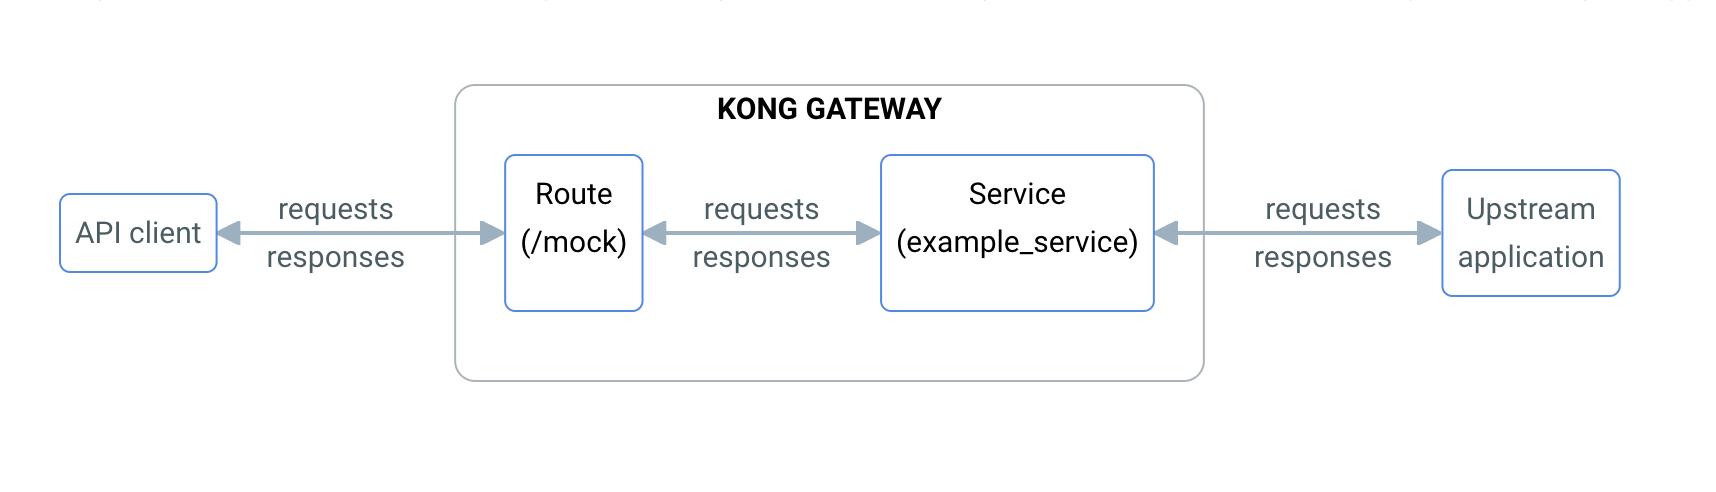
\includegraphics[width=\columnwidth]{images/kong-gateway.png}
  \caption{Kong Gateway - Rutas y servicios}
  \label{fig:kong_gateway_rutas_servicios}
\end{figure}

\subsubsection*{Servicio}
En Kong Gateway, un servicio es una abstracción de una aplicación upstream existente. 
Los servicios pueden almacenar colecciones de objetos como configuraciones de plugins y políticas, y pueden asociarse con rutas.

Al definir un servicio, se proporciona un nombre y la información de conexión a 
la aplicación upstream. Estos detalles de conexión pueden especificarse en un solo 
campo URL o separadamente en los campos de protocolo, host, puerto y ruta.

Los servicios tienen una relación de uno a muchos con las aplicaciones upstream, 
lo que permite crear comportamientos avanzados de gestión de tráfico.

\subsubsection*{Ruta}

Una ruta es un camino hacia un recurso dentro de una aplicación upstream. 
Las rutas se añaden a los servicios para permitir el acceso a la aplicación subyacente. 
En Kong Gateway, las rutas suelen mapearse a endpoints expuestos a través de la aplicación Kong Gateway. 
Además, las rutas pueden definir reglas que relacionan solicitudes con servicios asociados, 
lo que permite que una ruta pueda referenciar múltiples endpoints. Una ruta básica debe tener un nombre, 
una o varias rutas, y referenciar a un servicio existente.

% Fuentes: 
% https://docs.konghq.com/gateway/latest/
% https://docs.konghq.com/konnect/analytics/
% https://docs.konghq.com/gateway/latest/get-started/services-and-routes/

% \begin{thebibliography}{9}
% \bibitem{kong} Kong Gateway: Servicios y Rutas. \textit{KongHQ Documentation}. Disponible en: \url{https://docs.konghq.com/gateway/latest/get-started/services-and-routes/}
% \end{thebibliography}
\section{Amazon QuickSight}

Amazon QuickSight \cite{aws-quicksight} es una herramienta de inteligencia de negocio
basada en la nube capaz de escalar si así lo requiere, además que podemos combinar data de diferentes
orígenes.

Cuando tú tienes la correcta información en el momento correcto puedes tomar mejores decisiones.

Algunos de los beneficios: \
\begin{description}
	\item[In Memory Engine:] Guarda la data en memoria haciendo más rápida las consultas posteriores
	\item[Collaborative:] No hay necesidad de instalar alguna aplicación
	\item[Publish and Share:] Puedes compartir tus análisis como un dashboard
\end{description}

\subsection{¿Cómo trabaja?}
\begin{figure}[h!]
	\centering
	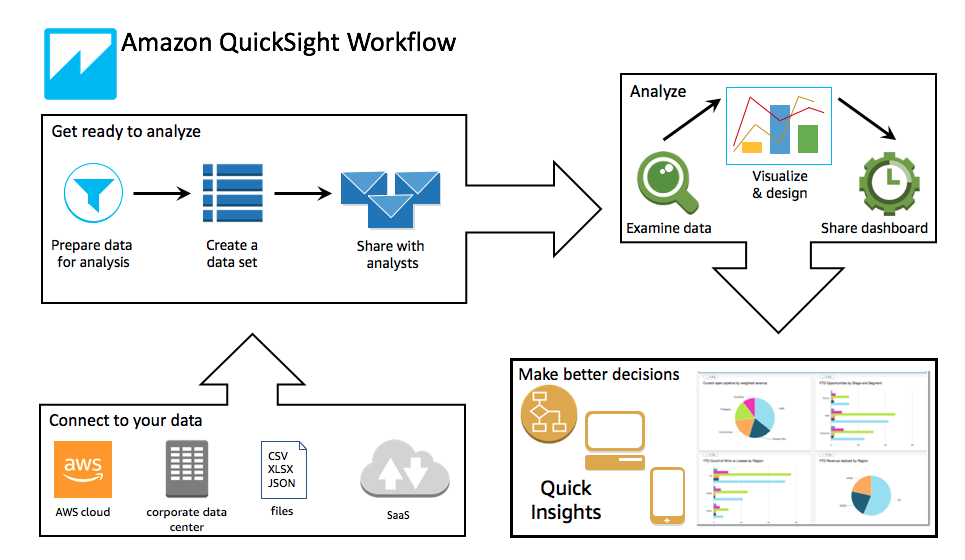
\includegraphics[width=\columnwidth]{images/aws_quicksight}
	\caption{Workflow QuickSight}
	\label{fig:quicksight_workflow}
\end{figure}

Tenemos que preparar la data para su respectivo análisis. Esto podría incluír hacer cambios en: \
\begin{itemize}
	\item Filtrar data que sea más relevante para ti
	\item Renombrar columnas para una mejor lectura
	\item Cambiar algunos tipos de datos por otros
	\item Creando una sql para refinar la data.
\end{itemize}

\subsection{Orígenes de data soportados}
Podemos usar: \
\begin{itemize}
	\item Amazon Athena
	\item Amazon Aurora
	\item Amazon Redshift
	\item Amazon S3
	\item Apache Spark
	\item Google Bigquery
	\item Mysql
\end{itemize}

\subsection{Actualizando la Data}
Hay 2 maneras: \
\begin{description}
	\item[Direct Query:] Si usas esta opción cada vez que tu ingreses al dashboard tu verás que la información está actualizada
	\item[SPICE:] No se actualiza, tienes que de forma manual, eliminar el dataset y volver a crearlo para que pueda tomar la información de nuevo.
\end{description}

\subsection{Precios y Límites}
Cuenta con los siguientes planes: \
\begin{description}
	\item[Standard Edition:] Cobro por usuarios y existe una tarifa base, ideal para pequeños equipos o empresas que necesitan crear informes o dashboards básicos
	\item[Enterprise Edition:] Cobro basado en sesiones, una sesión se considera la visita al sitio en un rago de 30 min, tarifa por usuario lector, tienes acceso a mas herramientas de ML, Active Directory
\end{description}

\section{Looker Studio}
Looker Studio es una herramienta sin coste que convierte tus datos en informes y paneles
claros, totalmente personalizables y fáciles de consultar y compartir. \cite{looker-data-visualization}

\subsection{Características}
En Looker Studio podemos encontrar las siguientes características:

\subsubsection{Interfaz web sencilla}
Looker Studio está diseñado para ser intuitivo y fácil de usar. El editor de informes
incluye objetos que se pueden arrastrar y soltar fácilmente, con paneles de propiedades
totalmente personalizados y un lienzo a la cuadrícula.

\subsubsection{Plantillas de informes}
Gracias a una sólida biblioteca de plantillas de informes entre las que elegir, puedes
ver tus datos en cuestión de minutos. Conecta tus fuentes de datos y personaliza el
diseño según lo que necesites.

\subsubsection{Data Connectors}
Las fuentes de datos sirven para conectar informes de Looker Studio con datos subyacentes.
Cada fuente tiene un conector único y prediseñado para garantizar que el acceso y el uso
de datos sea fácil.

\subsubsection{API de Looker Studio}
La API de Looker Studio permite a las organizaciones de Google Workspace o Cloud Identity
automatizar la gestión y la migración de recursos de Looker Studio. Puedes configurar
una aplicación para usar la API de Looker Studio de forma rápida y sencilla.

\subsubsection{Inserción de informes}
Si insertas tu informe de Looker, podrás incluirlo en cualquier página web o intranet
para que te sea más fácil contar tu historia a los equipos o al resto del mundo.
\section{Benchmark}


\begin{table}[H]
\centering
\caption{Benchmark de Features y Capacidades entre Kong y Amazon API Gateway}
\label{tab:benchmark}
\begin{tabularx}{\linewidth}{|X|X|X|}
\toprule
\textbf{Descripción} & \textbf{Kong} & \textbf{Amazon API Gateway} \\
\midrule
\small \textbf{Escalabilidad} & \small Escalabilidad horizontal a través de una arquitectura distribuida. & \small Escalabilidad automática con integración perfecta con los servicios de AWS. \\
\midrule
\small \textbf{Personalización} & \small Amplias opciones de personalización mediante su arquitectura de plugins. & \small Experiencia más simplificada con menos opciones de personalización. \\
\midrule
\small \textbf{Monitoreo y Analítica} & \small Integración con diversas herramientas de terceros para monitoreo y analítica. & \small Análisis detallado mediante AWS CloudWatch. \\
\midrule
\small \textbf{Integración} & \small Soporte para una amplia gama de integraciones con servicios y herramientas externas. & \small Integración estrecha con el ecosistema de AWS. \\
\midrule
\textbf{Facilidad de Uso} & Requiere conocimientos técnicos para aprovechar completamente sus capacidades. & Interfaz fácil de usar, accesible para desarrolladores de todos los niveles. \\
\midrule
\textbf{Costos} & Estructura de precios flexible con versiones gratuitas y suscripciones para empresas. & Modelo de precios de pago por uso basado en el número de llamadas a la API, transferencia de datos y características adicionales. \\

\bottomrule
\end{tabularx}
\end{table}
\section{Conclusión}

Habiendo revisado de manera general las caracteristicas de ambos productos y
poninendo a prueba sus capacidades, recomendamos el uso de \textbf{Amazon API Gateway}
por las siguientes razones:
\begin{itemize}
  \item \textbf{Integración}
  \item \textbf{Facilidad de Uso}
  \item \textbf{Costos}
\end{itemize}
A su vez tambien reconocemos que el producto Kong podría ser una muy buena opción en
casos muy particulares, pero a nivel general recomendamos \textbf{Amazon API Gateway}


%%
%% The acknowledgments section is defined using the "acks" environment
%% (and NOT an unnumbered section). This ensures the proper
%% identification of the section in the article metadata, and the
%% consistent spelling of the heading.
% \begin{acks}
% To Robert, for the bagels and explaining CMYK and color spaces.
% \end{acks}

%%
%% The next two lines define the bibliography style to be used, and
%% the bibliography file.
\bibliographystyle{ACM-Reference-Format}
\bibliography{bibliography}


%%
%% If your work has an appendix, this is the place to put it.
\appendix

\end{document}
\endinput
%%
%% End of file `sample-sigplan.tex'.